% %% %%%%%%%%%%%%%%%%%%%%%%%%%%%%%%%%%%%%%%%%%%%%%%%%%%%%%%%%%%
% step-1.tex
%
% Author:  Mauricio Matamoros
% License: MIT
%
% %% %%%%%%%%%%%%%%%%%%%%%%%%%%%%%%%%%%%%%%%%%%%%%%%%%%%%%%%%%%

%!TEX root = ../practica.tex
%!TEX root = ../references.bib

% CHKTEX-FILE 1
% CHKTEX-FILE 13
% CHKTEX-FILE 46

\subsection{Paso 1: Alambrado}%
\label{sec:step1}%
%
\begin{wrapfigure}[16]{r}{0.33\columnwidth}
	\vspace{-8mm}
	\centering
	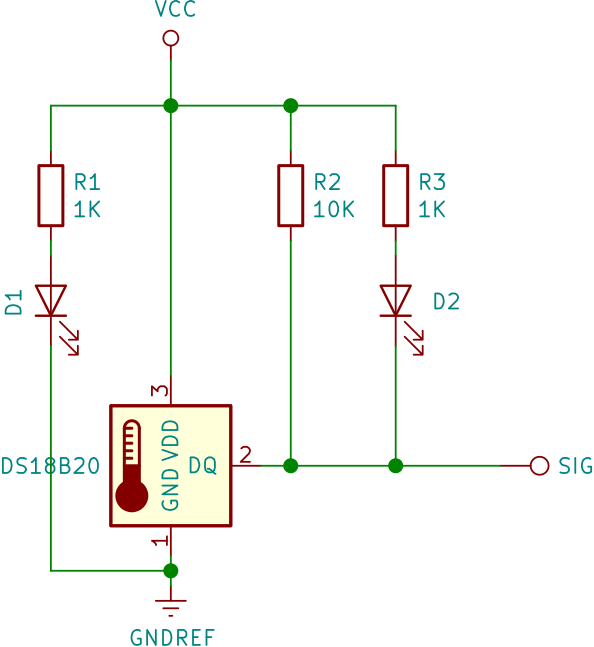
\includegraphics[width=0.3\columnwidth,height=7cm,keepaspectratio]{img/DS18B20.png}
	\caption{Alambrado del sensor de temperatura 1-Wire DS18B20}
	\label{fig:circuit-full} % CHKTEX 24
\end{wrapfigure}
%
El proceso de alambrado de esta práctica es relativamente simple y considera dos circuitos: el sensor DS18B20 y el display $LCD-16\times2$.
El primer circuito, mostrado en la \Cref{fig:circuit-full}, permite leer directamente del sensor de temperatura DS18B20 mediante el bus 1-Wire.
El segundo circuito (\Cref{fig:lcd}) consiste en la interfaz de conexión entre el $LCD-16\times2$ y el bus \IIC vía el módulo expansor de 8 bits a \IIC el PCF8574.

Alambre primero el circuito del sensor de temperatura DS18B20 mostrado en la \Cref{fig:circuit-full} consistente en el integrado DS18B20,
las dos resistencias de 1k$\Omega$,
los diodos emisores de luz
y la resistencia de pull-up de 10k$\Omega$.
Verifique que el diodo emisor de luz entre \textsc{Vcc} y tierra sea el \textsc{Led} \textcolor{red}{\textbf{ROJO}},
y que el diodo emisor de luz entre \textsc{Vcc} y \textsc{Sig} sea el \textsc{Led} \textcolor{OliveGreen}{\textbf{VERDE}}.
Finalmente, conecte los cables de \textsc{Vcc} y \textsc{Gnd} a la Raspberry Pi, así como el cable de datos \textsc{Sig} al pin número 7 (\textsc{Gpio4}).

\medskip
Tras alambrar el primer circuito realice el experimento prueba indicado en la \Cref{sec:step2}.
\medskip

A continuación ensamble el display al adaptador \IIC{} a $LCD-16\times2$ y conecte este último al bus \IIC de la Raspberry Pi como ilustran la \Cref{tbl:pi-arduino-i2c} y la \Cref{fig:lcd}.

\begin{table}
	\centering
	\caption{Conexiones \IIC entre la Raspberry Pi y el adaptador \IIC{} a $LCD-16\times2$}
	\label{tbl:pi-arduino-i2c} % CHKTEX 24
	\begin{tabularx}{0.8\linewidth}{cX rcl}
	\toprule
	\multicolumn{2}{c}{   Pin   } & \multicolumn{3}{c}{\multirow{2}{*}{Conexión}}  \\
	\multicolumn{2}{c}{Raspberry} & \multicolumn{3}{c}{}                           \\
	\midrule
	       3 & (GPIO2)            & Raspberry Pi SDA & $\rightarrow$ & Adaptador SDA \\
	       5 & (GPIO3)            & Raspberry Pi SCL & $\rightarrow$ & Adaptador SCL \\
	       6 & (\GND)             & Raspberry Pi GND & $\rightarrow$ & Adaptador GND \\
	       6 & (\GND)             & Raspberry Pi VCC & $\rightarrow$ & Adaptador VCC \\
	\bottomrule
	\end{tabularx}
\end{table}

Hay tutoriales que sugieren utilizar un convertidor de niveles de voltaje cuando se conecta una Raspberry Pi a un arduino mediante \IIC{}, especialmente cuando la Raspberry Pi opera a 3.3V. Esto \textbf{NO} es necesario cuando la Raspberry
Pi está configurada como dispositivo maestro o \emph{master}.

Esto es posible debido a que el adaptador no tiene resistencias de acoplamiento a positivo o \emph{pull-up} integradas, mientras que los pines \IIC de la Raspberry Pi están conectados internamente a la línea de 3.3V mediante resistencias de 1.8k$\Omega$.
Por este motivo, tendrán que quitarse las resistencias de \emph{pull-up} a cualquier otro dispositivo esclavo que se conecte al bus \IIC de la Raspberry Pi.\footnote{Para más información sobre el papel de las resistencias de acoplamiento a positivo o \emph{pull-up} en un bus \IIC se puede consultar \url{http://dsscircuits.com/articles/effects-of-varying-i2c-pull-up-resistors} }

\begin{wrapfigure}[6]{r}{5cm}
	\vspace{-8mm}
	\centering
	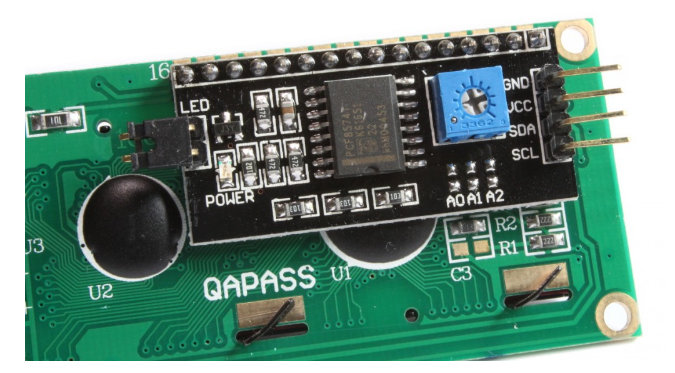
\includegraphics[width=\linewidth]{img/i2clcd.png}
	\caption[Adaptador \IIC acoplado a LCD]{Adaptador \IIC acoplado a display\footnotemark}%
	\label{fig:lcd} % CHKTEX 24
\end{wrapfigure}
\footnotetext{Imagen obtenida de \url{https://alselectro.wordpress.com/2016/05/12/serial-lcd-i2c-module-pcf8574/}}
